\documentclass[svgnames]{beamer}

\usetheme{Dresden}
\usecolortheme{beaver}

\usepackage{import, fancybox, graphicx, color}

\newcommand{\ssline}{\vspace{8 pt}}

\title{Transport Protocols \\for Gracefully Mobile Applications}

\author{Keith Winstein, Anirudh~Sivaraman, and Hari~Balakrishnan}
\institute{M.I.T.~CSAIL}
\date{November 15, 2012}

\begin{document}

\begin{frame}[plain]

\titlepage

\end{frame}

\begin{frame}
\frametitle{Outline}
\tableofcontents{}

\end{frame}

\section{Sprout: Flow control for interactive apps}

\begin{frame}
\frametitle{Mobile wireless networks are variable}

{\small
\def\svgwidth{\columnwidth}\input{allcapacity.pdf_tex}
}

\end{frame}

\begin{frame}
\frametitle{Videoconferencing systems work poorly on LTE}

\begin{itemize}
\item We measured cellular networks while driving:

\begin{itemize}
\item {\color{red}\bf Verizon LTE}
\item Verizon 3G (1xEV-DO)
\item AT\&T LTE
\item T-Mobile 3G (UMTS)
\end{itemize}

\item Then ran apps across emulated network:

\begin{itemize}
\item {\color{red}\bf Skype} (Windows 7)
\item Google Hangout (Chrome on Windows 7)
\item Apple Facetime (OS X)
\end{itemize}

\end{itemize}

\end{frame}

\begin{frame}
\frametitle{Why is performance so bad?}

\begin{itemize}
\item Exiting schemes \textbf{react} to congestion signals.

\begin{itemize}
\item Packet loss.
\item Increase in round-trip time.
\end{itemize}

\item This feedback comes too late to help.

\item The killer: \textbf{self-inflicted queueing delay}.

\item Any overshoot means a queue filling up with packets.

\end{itemize}

\end{frame}

\begin{frame}
\frametitle{Performance summary}
\vspace{-1 cm}
\def\svgwidth{\columnwidth}\footnotesize\import{dotgraphs/}{VerizonLTE-Uplink-stage0.pdf_tex}
\end{frame}

\begin{frame}
\frametitle{Sprout's goal}

\begin{itemize}
\item As much throughput as possible, with
\item bounded risk of delay $>$ 100~ms.
\end{itemize}

\end{frame}

\begin{frame}
\frametitle{Bounded risk of delay}
\begin{itemize}

\item \textbf{Infer} link speed from interarrival distribution.

\item \textbf{Predict} future link speed.

\begin{itemize}
\item Don't wait for congestion.
\end{itemize}

\item \textbf{Control:} Send as much as possible, but require:

\begin{itemize}

\item 95\% probability all packets will arrive within 100~ms.

\end{itemize}

\end{itemize}

\end{frame}

\begin{frame}
\frametitle{Infer link speed from interarrival distribution}

\def\svgwidth{0.7 \columnwidth}\input{vz-inter.pdf_tex}

\end{frame}

\begin{frame}
\frametitle{Predict future link speed}

\begin{itemize}
\item Count packets in every 20~ms tick.

\item Use Bayesian updating to infer (uncertain) link speed.

\item Make a cautious forecast.
\end{itemize}

\end{frame}

\begin{frame}

\begin{centering}
\def\svgwidth{0.85 \columnwidth}\input{sprout-model.pdf_tex}

\end{centering}

\end{frame}

\begin{frame}
\frametitle{The cautious forecast}

\begin{itemize}

\item Receiver has cloud of current link speeds

\item For eight 20~ms ticks in the future:

\begin{itemize}
\item Predict future link speed

\item Find 5th percentile of cumulative packets
\end{itemize}

\item Send forecast to sender (piggyback)

\item Most of the math is precalculated.

\end{itemize}
\end{frame}

\begin{frame}
\frametitle{Limitations}

\begin{itemize}

\item Stochastic model has not been tuned

\item Designed for cellular link with per-user queue

\item If other users can cause you big delay, can't solve end-to-end

\end{itemize}

\end{frame}

\begin{frame}
\frametitle{Verizon LTE uplink: head-to-head}

\end{frame}

\begin{frame}
\frametitle{Verizon LTE uplink}
\vspace{-1 cm}
\def\svgwidth{\columnwidth}\footnotesize\import{dotgraphs/}{VerizonLTE-Uplink-stage0.pdf_tex}
\end{frame}

\begin{frame}
\frametitle{Verizon LTE uplink}
\vspace{-1 cm}
\def\svgwidth{\columnwidth}\footnotesize\import{dotgraphs/}{VerizonLTE-Uplink-stage1.pdf_tex}
\end{frame}

\begin{frame}
\frametitle{Verizon LTE uplink}
\vspace{-1 cm}
\def\svgwidth{\columnwidth}\footnotesize\import{dotgraphs/}{VerizonLTE-Uplink-stage2.pdf_tex}
\end{frame}

\begin{frame}
\frametitle{Verizon LTE uplink}
\vspace{-1 cm}
\def\svgwidth{\columnwidth}\footnotesize\import{dotgraphs/}{VerizonLTE-Uplink.pdf_tex}
\end{frame}

\begin{frame}
\frametitle{Verizon LTE downlink}
\vspace{-1 cm}
\def\svgwidth{\columnwidth}\footnotesize\import{dotgraphs/}{VerizonLTE-Downlink.pdf_tex}
\end{frame}

\begin{frame}
\frametitle{Verizon 3G (1xEV-DO) uplink}
\vspace{-1 cm}
\def\svgwidth{\columnwidth}\footnotesize\import{dotgraphs/}{Verizon3G1xEV-DO-Uplink.pdf_tex}
\end{frame}


\begin{frame}
\frametitle{Verizon 3G (1xEV-DO) downlink}
\vspace{-1 cm}
\def\svgwidth{\columnwidth}\footnotesize\import{dotgraphs/}{Verizon3G1xEV-DO-Downlink.pdf_tex}
\end{frame}

\begin{frame}
\frametitle{AT\&T LTE  uplink}
\vspace{-1 cm}
\def\svgwidth{\columnwidth}\footnotesize\import{dotgraphs/}{ATTLTE-Uplink.pdf_tex}
\end{frame}


\begin{frame}
\frametitle{AT\&T LTE downlink}
\vspace{-1 cm}
\def\svgwidth{\columnwidth}\footnotesize\import{dotgraphs/}{ATTLTE-Downlink.pdf_tex}
\end{frame}

\begin{frame}
\frametitle{T-Mobile 3G (UMTS)  uplink}
\vspace{-1 cm}
\def\svgwidth{\columnwidth}\footnotesize\import{dotgraphs/}{T-Mobile3GUMTS-Uplink.pdf_tex}
\end{frame}


\begin{frame}
\frametitle{T-Mobile 3G (UMTS) downlink}
\vspace{-1 cm}
\def\svgwidth{\columnwidth}\footnotesize\import{dotgraphs/}{T-Mobile3GUMTS-Downlink.pdf_tex}
\end{frame}

\begin{frame}
\frametitle{Overall results}

\begin{tabular}{|l|c|c|}
\hline
{\color{blue}Sprout} vs.~ & Avg.~speedup & Delay reduction \\
\hline
\hline
{\color{red}Skype} & $2.2\times$ & $7.9\times$ \\
{\color{red}Hangout} & $4.4\times$ & $7.2\times$ \\
{\color{red}Facetime} & $1.9\times$ & $8.7\times$ \\
\hline
{\color{ForestGreen}Compound} & $1.3\times$ & $4.8\times$ \\
{\color{ForestGreen}TCP Vegas} & $1.1\times$ & $2.1\times$ \\
{\color{ForestGreen}LEDBAT} & Same & $2.8\times$ \\
{\color{ForestGreen}Linux TCP (CUBIC)} & $1.1\times$ & $79\times$ \\
%CUBIC/CoDel & & \\
%Compound/CoDel & & \\
\hline
\end{tabular}

\end{frame}

\begin{frame}
\frametitle{Competes with AQM even though end-to-end}
\vspace{-1 cm}
\def\svgwidth{\columnwidth}\footnotesize\import{dotgraphs/}{Codels.pdf_tex}
\end{frame}

\begin{frame}
\frametitle{Future work}

\begin{itemize}
\item Public contest for best predictor
\item Anybody will be able to build protocol using results
\end{itemize}
\end{frame}

\begin{frame}
\frametitle{Sprout for controlled delay over cellular networks}

\begin{itemize}
\item \textbf{Infer} link speed from interarrival distribution

\item \textbf{Predict} future link speed

\item \textbf{Control} risk of large delay

\item Yields 2--4$\times$ throughput of Skype, Facetime, Hangout

\item Achieves 7--9$\times$ reduction in self-inflicted delay

\item Matches active queue management \textbf{without router changes}

\end{itemize}

\end{frame}

\section{SSP: Graceful mobility}

\begin{frame}
\tableofcontents[currentsection]
\end{frame}

\begin{frame}
\frametitle{Motivation: frustration with SSH}

\begin{itemize}

\item Can't roam:

\begin{itemize}
\item \ldots across Wi-Fi networks.
\item \ldots from Wi-Fi to cell or vice versa.
\end{itemize}

\item Can't sleep and wake up (usually).

\begin{itemize}
\item \ldots TCP disconnects if unacked data for too long.
\end{itemize}

\item Responds poorly to packet loss.

\item All UI requires round-trip to server.

\end{itemize}

\end{frame}

\begin{frame}

\frametitle{Octet stream is wrong layer of abstraction}

\begin{itemize}
\item Client wants \emph{latest} screen.
\item After interruption, don't want to replay megabytes.
\item But SSH doesn't understand data, so must send everything.
\item TCP fills buffers, so Control-C takes forever.
\end{itemize}

\end{frame}

\begin{frame}

\frametitle{What we built}

\begin{enumerate}

\item Protocol for low-latency \textbf{object synchronization}

\begin{itemize}
\item with roaming
\item through suspend/resume
\item over lossy network paths
\end{itemize}

\item Supports \textbf{rolling latency compensation} on client side

\item Mobile shell application to replace SSH.

\end{enumerate}

\end{frame}

\begin{frame}

\frametitle{State Synchronization Protocol}

\begin{itemize}

\item Runs over UDP.

\item Instead of sending \emph{octet streams}, synchronize \emph{objects}.

\item Object must support:
\begin{itemize}
\item \texttt{diff}: make vector from state $A \rightarrow B$
\item \texttt{patch}: apply vector to $A$ to make $B$
%\item \texttt{subtract}: remove common prefix from $A, B$
\end{itemize}

\item Object implementation, \textbf{not protocol}, defines
  synchronization semantics.

\end{itemize}

\end{frame}

\begin{frame}
\frametitle{Secure quick roaming}

\begin{itemize}

\item Protected by AES-OCB (Krovetz 2011)
\begin{itemize}
\item Integrity and confidentiality with one key.
\end{itemize}

\item All packets are idempotent operations.

\item Unlike SSH or TLS, connection control is also authenticated.

\begin{itemize}
\item Attacker cannot terminate connection with FIN or RST.
\end{itemize}

\item Roaming is easy:
\begin{itemize}
\item Source address of latest authentic packet from client \\ $\Rightarrow$
server's new target
\item Client may not even \textbf{know} it has roamed.
\end{itemize}

\end{itemize}

\end{frame}

\begin{frame}
\frametitle{P$\cdot$retransmissions trade performance for robustness.}

SSP has options in choosing which \texttt{diff} to send:

\begin{enumerate}

\item Last ack was for state \#3. Then state changes to \#4.

\item Host sends \texttt{diff} from $3 \rightarrow 4$.

\item Object changes to state \#5.

\item If no timeout yet, make next \texttt{diff} as $4
  \rightarrow 5$.

\item \textbf{Also} make \texttt{diff} from $3 \rightarrow
  5$: the \emph{prophylactic retransmission}.

\item If p$\cdot$retransmission is shorter or not much longer, send instead.

\end{enumerate}

\end{frame}

\begin{frame}
\frametitle{Rolling predictions}

\begin{itemize}

\item Client runs predictive model of server UI.

\item Make predictions in \emph{epochs}.

\item If any from epoch $n$ is confirmed, show whole epoch.

\item If prediction from epoch $n$ is wrong, hide that epoch.

%\begin{itemize}
%\item $n$ might be current epoch or one from the past.
%\end{itemize}

\item If user does something difficult to handle, become
  tentative: \emph{increment epoch}.

\item Better than Meteor's on/off ``local mode.''

\end{itemize}

\end{frame}

\begin{frame}

\noindent 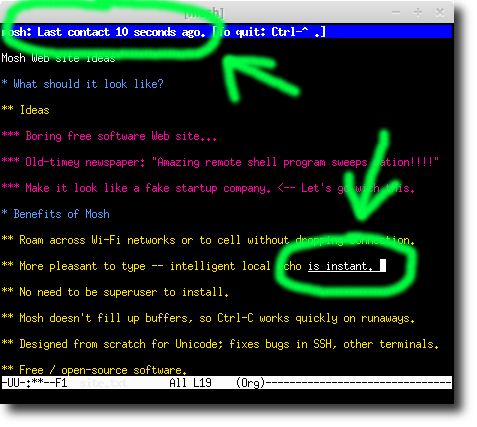
\includegraphics[scale=.5]{mosh.png}

\end{frame}

\begin{frame}
\frametitle{Demo}

\end{frame}

\begin{frame}
\frametitle{Deployment}

\begin{itemize}
\item In Debian, Ubuntu, Fedora, Gentoo, Arch, Slackware.

\item Available for Red Hat, CentOS, Oracle Linux.

\item In MacPorts, Homebrew, FreeBSD ports collection.

\item Works on Cygwin, Solaris, experimental port to Android.

\item Cover of Linux Magazine this month (Nov.~2012).

\item Top repository of the month on GitHub.

\item 300,000+ page views, 75,000+ downloads, 1,500+ VCS followers.

\end{itemize}

\end{frame}

\begin{frame}
\frametitle{Gmail app if user roams at the wrong time}

\textbf{July 5, 2012}:\\
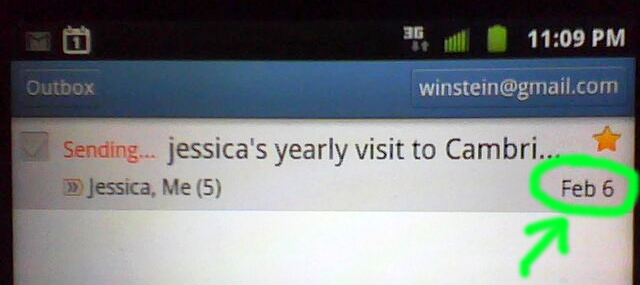
\includegraphics[scale=.5]{gmail.png}

\end{frame}

\begin{frame}
\frametitle{State synchronization for all}

Many Web and native apps have trouble with roaming and intermittent connectivity:

\begin{itemize}
\item Android Gmail app
\item Skype
\item Google Chat
\item gmail.com
\item quora.com
\item Google Voice
\item Twitter
\end{itemize}

These problems may also be expressed as state synchronization.

\end{frame}

\section{Alfalfa: video for varying networks}

\begin{frame}
\tableofcontents[currentsection]
\end{frame}

\begin{frame}
\frametitle{Coded video is also a state synchronization problem}

\begin{itemize}

\item P-pictures are ``diff'' from previously-sent frame.

\item B-pictures are ``diff'' from two previously-sent frames.

\end{itemize}

\end{frame}

\begin{frame}
\frametitle{Mobile video conferencing}

For reliable mobile video conferencing, application wants from:

\begin{itemize}
\item \textbf{Network}: ``How much is it safe to send now?''

\begin{itemize}
\item TCP and DCCP don't supply this.
\end{itemize}

\item \textbf{Video encoder}: ``Give me a P-picture from this frame
to \emph{this} frame with maximum length $x$.''

\begin{itemize}
\item x264 (H.264) and libvpx (VP8) don't do this.
\end{itemize}

\item \textbf{Video decoder}: ``Apply this P-picture to \emph{this}
predicate picture, and give me the results.''

\begin{itemize}
\item QuickTime, libavcodec, etc.~don't allow this.
\end{itemize}

\end{itemize}

Solution: Sprout/SSP and ``explicit-state'' video codec API.

\end{frame}

\begin{frame}
\frametitle{Video complications}

\begin{itemize}
\item P-picture is not just based on predicate \emph{frame}.

\item Also have quantization tables, probability tables, other
  inter-frame state.

\item Specifications don't envision this use.

\item Aren't explicit about what state needs to be carried across
  frames.

\end{itemize}

So far, we have implemented API for MPEG-2 video.

\end{frame}

\begin{frame}
\frametitle{What about Netflix / YouTube?}

Current practice:

\begin{itemize}
\item encode multiple quality levels, each with VBV.

\item player can switch, but requires I-picture and visible jump.

\item often switch only available every 10 seconds!
\end{itemize}

Our view:

\begin{itemize}
\item VBV was designed for isochronous broadcast channels!

\item Ditch VBV: the player's buffer is all that matters.

\item Encode full trellis of diffs between quality levels.

\item \textbf{Let the decoder choose} how it wants to plan ahead.

\item Can run over HTTP.
\end{itemize}

\end{frame}

\begin{frame}
\frametitle{Conclusion}

\begin{itemize}

\item Sprout: end-to-end flow control for cellular networks that
  matches or outperforms in-network modifications.

\item SSP: protocol for gracefully mobile state synchronization.

\item Alfalfa: video for varying networks.

\end{itemize}

\end{frame}

\end{document}
